\section{Camera Calibration and Augmentation}

This section is divided into two parts, first we will look at how we obtained proper camera calibration and distortion coefficients. Then we look at how we used this information to augment the image obtained from the camera with a projected cube.

\subsection{Camera Calibration}

During the camera calibration phase we aim to obtain intrinsic camera parameters. This is divided into two parts, first there is a camera matrix K (see Equation \ref{eq:cameramatrix}) which describes the intrinsic properties of the camera, and then there are distortion coefficients which we do not represent in the linear camera model, but they affect the image nonetheless. 

The R|t part is the rotation/translation matrix. This are the extrinsic properties of the camera like its rotation and translation in the world.

P is a point in the 3D space that we want to project onto the 2D image obtained by the camera. 

C represents the 2D coordinates in the image produced by the camera when P is projected.

\begin{equation}
	\underbrace{
		\begin{bmatrix}
			u \\
			v \\
			1
		\end{bmatrix}
	}_\text{C}
	=
	\underbrace{
		\begin{bmatrix}
			f_{x} & 0 & t_{x} \\
			0 & f_{y} & t_{y} \\
			0 & 0 & 1
		\end{bmatrix}
	}_\text{K}
	\cdot
	\underbrace{
		\begin{bmatrix}
			R_{1,1} & R_{1,2} & R_{1,3} & t_{x} \\
			R_{2,1} & R_{2,2} & R_{2,3} & t_{y} \\
			R_{2,1} & R_{2,2} & R_{3,3} & t_{z}
		\end{bmatrix}
	}_\text{R|t}
	\cdot
	\underbrace{
		\begin{bmatrix}
			X \\
			Y \\
			Z \\
			1
		\end{bmatrix}
	}_\text{P}
	\label{eq:cameramatrix}
\end{equation}

The calibration is obtained in OpenCV by repeated exposures containing the calibration pattern. Based on this, OpenCV calculates the intrinsic camera properties and returns them as K and distortion coefficients. It should be noted that unless the camera allows for focal length manipulation, the intrinsics will not change. So it makes sense to just calibrate once and save the calibration into a file which then can be reused.

\subsection{Augmentation}

In the next part we have used the calibration obtained in the previous section to augment the image with a 3D object (cube) Figure \ref{fig:augment}. The basis for this was to obtain a homography from one virtual camera to another. 

\begin{figure}[h!]
	\centering
	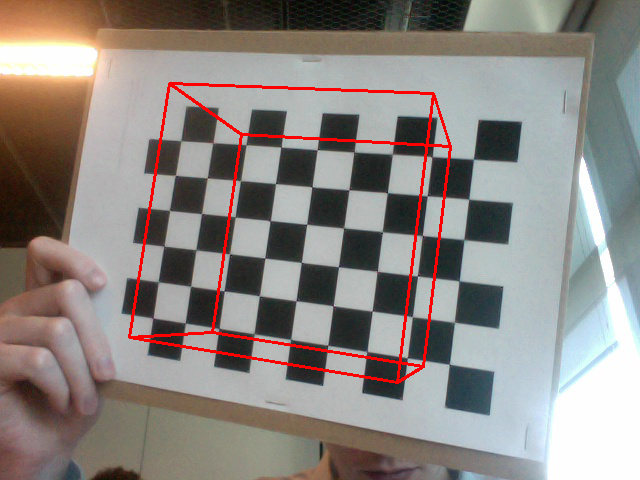
\includegraphics[width=\textwidth]{Handin2/images/augmentation1.png}
	\caption{Augmented image}
	\label{fig:augment}
\end{figure}

First we have constructed a camera that would look at just the chessboard pattern. Then we have calculated the positions of some select corners in that pattern, and using the same corners in the same pattern in the image obtained from the video, we have been able to estimate a homography that would describe the relationship between the two.

From that we have been able to re-construct the camera that was essentially used to take the video image. we have had the calibration from before, and now using the homography we have been able to calculate the rotation and translation matrices from the Equation \ref{eq:solvingforrotation} where we obtain $r_{1}$, $r_{2}$ and t as dot product of the inverse of K, the calibration matrix, and H, the homography between the two planes. $r_{3}$ can be calculated as a cross product of $r_{1}$ and $r_{2}$.

\begin{equation}
	K^{-1}H = [r_{1}, r_{2}, t]
	\label{eq:solvingforrotation}
\end{equation}

Now using the projection matrix of the second camera, we can project points in the 3D space onto the final image, so that they appear as if they were in the scene. And since the homogrpahy is calculated from one chessboard to another, the points are anchored the position of the chessboard.

